\newpage
\subsection{Migration of virtual networks with SDN}
In this section, we discuss the different virtual network migration solutions.
We start by presenting solutions published on the same year as OpenFlow and that have been used as a reference in a majority of SDN-based migration solution.

\subsubsection{Preliminary work}

\paragraph{VROOM}
Virtual ROuters On the Move (VROOM)~\cite{VROOM-Wang2008} is an early work about how the migration of virtual routers should be implemented on top of the physical infrastructure. 
VROOM outlines that most of the network state changes are caused by planned maintenance.
Moreover, power consumption is also a primary concern because efficient migrations can save up to hundreds of millions of dollars.
In this regard, VROOM presents a network virtualization and migration technique aiming at minimizing these costs and the duration of maintenance.
VROOM is composed of 3 building blocks: router virtualization, data and control plane separation, and dynamic interface binding.
Router virtualization is already implemented in some commercial routers, and VROOM presents two prototypes, one software based and the other one hardware based.
Data and control plane separation is achieved by using different virtualization environments (VE) in a virtualization infrastructure, namely OpenVZ~\cite{openvz}.
The data plane is implemented using OpenVZ first VE (VE0) in which the software implementation of the VROOM router will use a Linux kernel in a commodity server while the hardware implementation will use a NetFPGA circuit.
The control plane is also implemented using OpenVZ but using separate VEs (VE1, VE2, ...).
Each virtual router is stored in a VE, in which a kernel and routing protocol are implemented using a software suite.
The dynamic binding of the physical and virtual interfaces is divided into two main functions.
The first one implements the mapping of the virtual router with the corresponding Forwarding Information Base (FIB) inside the physical router.
The second one is the mapping of the FIB of the physical router with a corresponding physical interface.

\paragraph{Virtual Network Embedding and path migration}
Yu~\etal proposed in~\cite{VNE-Yu2008} a VNE model designed to support the splitting of a virtual link over several physical links, as well as dynamic virtual network reconfiguration.
The whole work is intended to improve resource allocation and maximize the acceptance rate. 
Path splitting takes a virtual link with a required amount of bandwidth that cannot be embedded on the physical infrastructure, and divides it into several smaller links that can be accepted by the infrastructure.
Path migration extends the usability of path splitting by allowing to recalculate the embedding of existing virtual networks and freeing extra resources otherwise not available using path splitting solely.
Authors provide an extensive evaluation of their mapping and migration algorithms using a simulator~\cite{vnesimulator}.

Both~\cite{VROOM-Wang2008} and~\cite{VNE-Yu2008} have been published on the same year as the publication of OpenFlow~\cite{Openflow-McKeown2008}, an implementation of the Software Defined Network paradigm that will become the standard of SDN for both industry and academia.
Despite the fact that these publications are not based on SDN, they lay grounds for plenty of the works we will now describe.

We divide the existing VN migration solutions based on the research issue they tackle to identify the existing lacks in the study of the migration process.
We summarize these issues into three categories: whether the solution is designed to improve the performance of the infrastructure, whether it was implemented to explore technical limitations on a virtualization platform or finally if it tackles a specific security problem.

\subsubsection{Improving the performance of the infrastructure}
Ye~\etal propose in~\cite{Ye2017a} a resource utilization model in which they aim to maximize the resource allocation on switches while looking to determine controllers that can be shut down due to underutilization and migrate switches.
Authors solve the resource allocation problem using optimization under constraints techniques. 
The switch migration problem is described as NP-hard and is approximated using a Log-sum-exp approximation.
This approximation determines the allocation of network switches on controllers that will maximize their utilization. 
From this distribution, authors construct a Markov chain that represent the different distributions strategies and where transitioning from a state to another corresponds to migrating a switch from a controller to another controller.

In~\cite{Wang2017d}, Wang \etal study a problem similar to~\cite{Ye2017a}, but are more focused on the migration and its efficiency, and present a Switch Migration-based Decision Making (SMDM) scheme. The problem is divided into three parts: detecting the overload of the controller due to an excessive amount of OF requests, the modeling of the migration's performance and finally, modeling the trade-off between the profit generated by the migration and the cost it incurred.
The overload detection correlates two types of information to determine overloaded controllers.
The first one is the actual amount of requests received by controllers, while the second is the load ratio between each pair of controllers.
This ratio is then bound to a threshold above which a migration will be triggered to relieve one controller from its load and reallocate it to the other.
Modeling the efficiency of the migration considers both the load variation of the controllers as well as the overhead of messages exchanged to implement the migration.  
Finally, the migration strategy is in charge of determining which switch should be selected as the next candidate for the migration and where it should be migrated.
Figure~\ref{fig:smdm-wang2017d} illustrate the interactions of the different components of the solution.

\begin{figure}[ht]
    \centering
    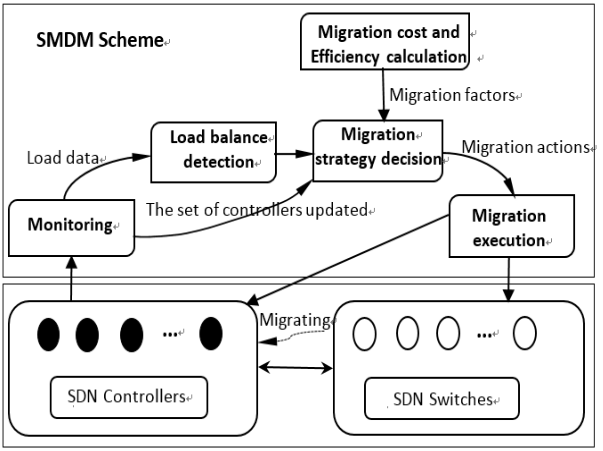
\includegraphics[scale=0.65]{figures/wang2017d.png}
    \caption{Architecture of the SMDM scheme~\cite{Wang2017d}}
    \label{fig:smdm-wang2017d}
\end{figure}

Lo~\etal introduce in~\cite{vnm-lo2013} the design of a virtual network migration process.
The cost of the migration is based on two metrics, the completion time of the migration as well as the bandwidth consumption.
Based on the original embedding and the new destination substrate, the goal is to determine the ordering of node migration that will minimize the cost of the migration.
For each step in the migration, the time taken to migrate a node is divided into two parts. The first one represents the time taken to prepare the migration and the second one is the time taken to actually transmit the different information to the destination substrate.
The cost of a migration step is the product of the time it takes to migrate the information and the impact the migration incurs on the bandwidth.
Virtual nodes are categorized based on whether the node has been migrated, if it will be at this step of the migration or if it will be later.
Similarly, the virtual links' are divided into three categories, whether the nodes composing the links have been migrated, will be migrated or will not be migrated.
The categorization of virtual resources is then used to determine the cost of the migration.
Three different virtual network migration algorithms are presented, differentiated by the fact that nodes may be either migrated one node at a time or multiple nodes may be migrated together.
The first algorithm is a greedy iteration over the individual costs of migrating each nodes.
The second algorithm is designed to minimize the migration time. Since migrated nodes are constrained not to be a neighbour of any other node, the algorithm determines the biggest set of independent nodes.
Then, the algorithm leverages the fact that several nodes can be migrated simultaneously to reduce the total migration time.
The third algorithm is a combination of the first two, where a tradeoff between migration time and migration cost is sought. The algorithm computes the different sets of independent nodes, and instead of choosing the largest one, choose the set with the smallest cost.
Again, this algorithm uses the simultaneous node migration to choose the set with the smallest cost.

Robust virtual network migration is studied in~\cite{Ko2017c}. Authors outline that traditional migration suffers from down times proportional to the size of the migrated virtual networks, while protection mechanisms cannot be adapted to support the dynamic changes in the network.
Three requirements are defined while considering drawbacks of existing migration techniques. 
First, the tenant's controller should never be notified of the migration.
Second, the migration process should account for the network traffic status inside the physical infrastructure.
Finally, the migration process should minimize the number of interactions between the network hypervisor and the physical infrastructure.
Protection and restoration techniques are described to account for these requirements.
Protection consists in deploying backup paths on the physical nodes, calculated prior to any incident.
This way, in case of a failure the traffic can immediately be routed through the alternative path. 
This method implies that the hypervisor must maintain regularly updated backup paths in each node, incurring computational overhead, bandwidth consumption as well as limitations on the physical resources of the switch.
Restoration is the case where all the backup paths are stored inside the network hypervisor and only deployed in case of a failure.
This method is based on the assumption that failures will rarely happen, thus the method being resource effective because it will not generate an important number of messages between the infrastructure and the hypervisor.
The network hypervisor determines a backup path that will minimize the the amount of messages sent to the infrastructure.
To do so, the backup path must use the same links as the original while only differing at the failure point.
Updates of backup paths are performed regularly while a monitoring device collects statistic on available resources to determine if the current backup paths can still be used.
The migration solution is implemented using OpenVirteX~\cite{OpenVirteX-Al-Shabibi2014}, where the path calculator and storage mechanisms are adapted to fit the new requirements. 
% Then new components related to the prioritization of backup paths, updating existing paths and monitoring the physical network are implemented and integrated into the hypervisor.

Improving the revenue generated with network virtualization can be done through migration.
In~\cite{fragment-Liu2018}, the purpose of VN migration is to optimize the acceptance ratio of new virtual network requests as well as the revenue to cost ratio.
While traditional VNE algorithms only rely on the individual capacities of nodes and links, they do not consider nodes with the bandwidth of adjacent virtual links.
To this end, the notion of fragment degree for a virtual node is introduced and is defined as a weighted combination of the CPU consumption ratio of the virtual node on its embedding node and the bandwidth consumption ratio of adjacent virtual links on the physical substrate.
The fragment degree of each virtual node is then associated with the embedding cost of existing virtual networks into a multi-objective integer linear program. The solution of this program being NP-hard to solve, authors make it computationally tractable with a novel algorithm: Fragment-aware Virtual network Reconfiguration (FA-VNR).
This algorithm first defines a migration trigger. 
% Maximizing revenue over time pushed for a periodical migration of VNs.
Then, it determines which set of physical nodes must be reconfigured by computing a dynamic threshold of ``fragmentation" in the infrastructure.
Similarly, the algorithm determines a set of virtual nodes to migrate based on their economical performance.
Once the destination substrate has been chosen, virtual nodes will be migrated and each virtual link connected to them will be redeployed using a shortest path algorithm.

\subsubsection{Evaluating virtualization platforms}
We present here two migration solutions that have been implemented on a particular physical infrastructure.
While~\cite{Lo2014} is not specifically designed to work on an SDN infrastructure, the problems and challenges it explores remain valid in the SDN paradigm.
Both solutions aim at outlining the technical limitations faced when migrating VNs.

\paragraph{PlanetLab}\textbf{\\} 
PlanetLab~\cite{planetlab} (PL) is a virtualization infrastructure used to provide slices of network resources for research experiments. Lo~\etal state in~\cite{Lo2014} that VN migration is a field where practical implementation and evaluation remain to be explored. They proposed a migration scheme and implemented it in PL, namely PL-VNM. This process should be designed to be automated, fast and to minimize the service disruption time. While the migration process is automated, there is no detection component to automatically trigger the migration. Due to technical limitations of PL it is impossible to migrate a VN from a slice to another. An alternative is proposed by partitioning the resources within a slice thus defining new virtual networks inside a PL slice and limiting the migration to the VNs created in a single slice. Virtual routers are instantiated for each virtual node required by the topology, and use an API to install forwarding rules in the kernel space of the physical node.
Authors proprose a simple migration algorithm based on the size of the flows to migrate.
The migration process consists in cloning the network state of virtual nodes (\ie FIB) and then  redirect VMs' traffic through the newly created virtual network.
While the duplication of networking state does not cause any packet loss from the tenant's point of view, setting up the redirection is most likely to create service disruption.
Two different approaches are taken and evaluated.\\
The first approach consists in preparing the scheduling for the host redirection and then sequentially send commands to the gateways connected to the hosts, namely remote scheduling.
Figure~\ref{fig:plvnm} depicts the modules of PL-VNM and how the migration process is handled.
One of the drawbacks of this method is the delay existing between the migration instruction being sent by the controller and the instruction actually being run at the gateway.\\
The second approach relies on determining the migration ordering and then scheduling the migration in the gateway using the UNIX command \textit{at}. The \textit{at} command makes sure that the migration is performed on time by synchronizing the gateway via the NTP protocol. Here, the potential latency to execute the migration is based on the time it takes for NTP to trigger \textit{at} and on the load of the gateways' CPU.
Both approaches make it hard to have a full control over the migration's timing.
Authors conclude with three recommendations for the PL infrastructure and in general for network hypervisors.
First, enabling gateway task scheduling with a magnitude order of milliseconds. As is, \textit{at} scheduling uses seconds for tasks triggers while path latency of remote scheduling is a few hundreds of ms.
Then, allowing the migration scheduler to prioritize migration commands to reduce the delay induced in the actual start of the command.
Finally, implementing asymmetric packet routing inside the infrastructure.
Because of the routing mode used in PL, each link in the gateway must have the same physical source and destination, thus preventing an asymmetric migration of the FIB from being effective. 

\begin{figure}[ht]
    \centering
    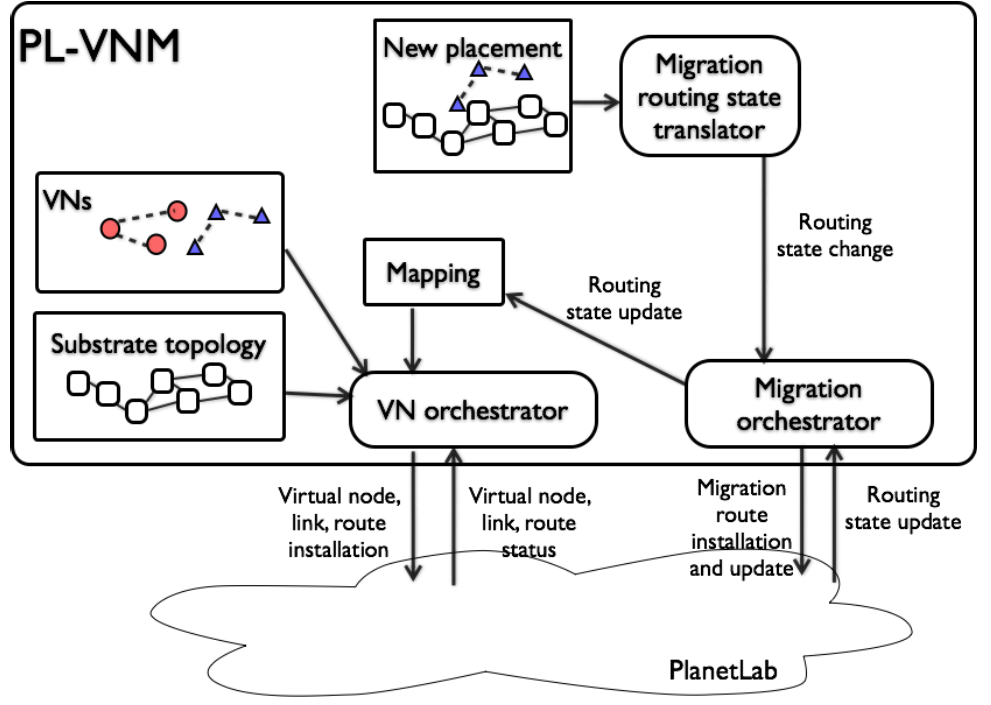
\includegraphics[scale=0.5]{figures/pl-vnm.png}
    \caption{Architecture of PL-VNM~\cite{Lo2014}}
    \label{fig:plvnm}
\end{figure}

\paragraph{GENI} \textbf{\\}
The GENI platform~\cite{GENI-Berman2014} is a network infrastructure based on SDN and used to provide isolated environments for researchers to run experiments.
Zhao~\etal propose in~\cite{Zhao2017} a VN migration scheme implemented using GENI. 
Similarly to PlanetLab, GENI has not been designed to support the migration of VNs over different physical substrates. 
We differentiate \textbf{slice} from \textbf{Virtual Networks (VN)} in~\cite{Zhao2017}.
A \textbf{slice} is a GENI slice, \ie the set of resources allocated to a tenant, while \textbf{VN}  are a subset of these resources.
Implementing VNs (original and migration backups) can be done by allocating all required resources to a single slice. This approach comes with drawbacks however: no clear isolation between VNs, lack of flexibility in case there is a need for a topology change and finally, in case of a failure of a VN or a host, the whole topology must be rebuilt.
Another approach consists in allocating one slice for a single VN and then, when migrating it allocate a new slice. The main challenge is to set up communication between the old and the new slice during the migration, since GENI enforces isolation between its slices.
In addition to the inter-slice communication, the migration process should not cause packet loss and be invisible to the tenant.
A proposed approach separates the old VN, the new VN and the VMs by setting up a different slice for each group. Two extra gateways are inserted in the VMs' slice, each connected to one of the other slices.
Without these gateways, the learning switch implemented by GENI would not allow to connect the hosts to the new VN because of conflicting rules (same source/destination, different output ports).
The three slices will then share a common VLAN to communicate together.
In order to minimize the packet loss incurred by the migration, the migration is optimized by scheduling the sequence of flows that will be deployed on the physical substrate.
First the rules between gateways and the new VN are set up, then the hosts' traffic is redirected towards the second gateway and finally old VN rules are dropped leading to a full disconnection of the former VN.
A problem similar to the migration with PlanetLab is how the migration is scheduled on the physical switches.
The first option is to remotely control network interfaces using SSH.
An SSH connection with each switch is established and old interfaces will be shut down while activating the new ones.
However, the latency induced by SSH authentication and by the time it takes to transmit commands makes the migration unpredictable.
On the other hand, the migration can be done by sending OF rules as the migration progresses. This method is deemed faster than the other one because it does not use SSH and its authentication overhead but it is also less secure.
Finally, the transparency of the migration is ensured by the migration controller who will act as a proxy between VNs and switches, intercepting packets and rewriting header fields to maintain a consistent view of the network.

\subsubsection{Formal verification and security}
In complement to the works aiming at improving the performance and the scalability of the virtualization infrastructure and the migration process, we now consider the works taking a formal approach to study specific properties of the migration process or using the migration process for security purposes.

\paragraph{Inter-flow consistency}\textbf{\\}
In an SDN infrastructure, the configuration deployed on SDN switches will be updated and evolve regularly. Such modifications are invoked by the SDN controller and deployed among several switches.
Flow consistency ensures that each flow will be processed by either the old or the new configuration all along the way, and not by a combination of the two.
However, Liu~\etal argue in~\cite{Liu2015a} that making sure that each individual flow has its own consistency preserved is not enough to respect certain security and reliability requirements.
It becomes necessary to model relationships between flows and to preserve certain properties throughout the migration.
The properties considered here are spatial isolation and version isolation.
The spatial isolation of two flows consists in preventing them from sharing a common physical resource before, during and after a change in the network configuration.
For instance, a critical flow carrying important information should not share a link with a certain traffic that may be subject to surges, thus leading to link congestion and the important flow not being delivered. Another case would be when attackers would try to intercept information on critical flows and then exploit the infrastructure.
Version isolation ensures that a configuration affecting different flows is fully deployed and prevents one flow being processed with one configuration and another flow with another version of the configuration.
This problem is related to the delay in actually deploying the configuration inside the switches, as outlined with PlanetLab and GENI.
The spatial isolation problem is approached using a dependence graph. Each path taken by a flow is mapped with the physical nodes they go through. Then, in case of overlapping node for several flows, the node is seen as a mutex node (similarly to the mutex of an operating system).
No flow may go through a mutex node if another flow is currently using it.
This ensures that specific traffic may not cohabit inside the same physical resources.
To ensure the version isolation of different flows, the system identifies the set of flows that must be isolated. Then, it picks one to be processed normally and forward to the controller all the traffic of the remaining flows. This way, it makes sure that there are not two flows being processed by 2 different versions of a configuration. And when all the cached traffic is re-injected inside the infrastructure, it is being processed by a fully updated networking state.
The generation of the dependence graphs is done by categorizing flows into two classes and using a greedy algorithm to determine how to minimize the amount of packet caching that would be done at the controller.
The ordering of the migration sequences is determined from the graph. Each sequence is composed of several configuration modification, and these modifications are also ordered to minimize the migration time. 

\paragraph{Moving Target Defense}\textbf{\\}
Dynamically changing the location of sensitive targets is a technique called Moving Target Defense (MTD). Such changes prevent an attacker from accurately knowing the attack surface of the system he is attacking. 
% because the configuration regularly changes. 
Chowdhary~\etal~\cite{Chowdhary2016} use MTD techniques as part of a Detect-Analyze-Counter cycle inside an SDN-based Cloud infrastructure. 
The security system is composed of four modules: a detection module, a vulnerability analyzer, a counter-measure creation and deployment component and a policy conflict resolution.
The detection module is in charge of gathering information about the vulnerabilities in the infrastructure.
Then, the analyzer will use these information to dynamically generate an attack graph representing the capacities of the attacker. 
A counter-measure will then be generated to mitigate the potential attacks and propose it to the conflict resolution module that will determine if the newly created counter-measure is not going to have harmful side effects. Once the counter-measure is accepted it is deployed in the infrastructure and the detection module is notified of the new configuration. This cycle approach creates a dynamic detection/mitigation environment.
The attack detection aspect is left out in this paper, as it is already a widely explored topic.
A well known drawback of attack graphs is the difficult scalability when the number of states grows.
This problem makes the graph generation computationally intractable. Partitioning the attack graph into smaller regions based on each tenant using the infrastructure simplifies the generation.
These sub-attack graphs are then simply merged together for the counter measure to be generated.
The counter-measure component determines which VM should be migrated based on a security score based on the CVSS Base Score.
Once the target VM is chosen, new flow rules are computed to implement the migration. 
The conflict resolution inspects the flow rules that should be deployed and extracts the actions of each rule and verify that they do not overlap with other existing flow rules. If a conflict arises, this module will try to find alternative rules. In the event where this would not be possible, the proposed counter-measure is rejected and a new one is computed.

\paragraph{Seamless migration}\textbf{\\}
In the previous works, minimizing the service disruption caused by the migration has always been a major concern in the design of the solution. However, while the efficiency of the solution was evaluated with various experiments, there was no formal approach describing the transparency of the migration and ensuring that no disruption of service will be experienced by a tenant.
The topic of seamless migration is brought up in~\cite{toward-Ghorbani2014} where Ghorbani~\etal take a closer look at network virtualization using SDN techniques.
Precisely, the focus is put on the one-to-many mapping, also known as the `Big Switch" abstraction.
Distributing a single virtual resource over several physical one may not preserve the per-flow correctness.
Similarly to the version isolation presented in~\cite{Liu2015a}, flow correctness considers flows individually and ensures that each packet of each flow  is always processed by one specific version of a network configuration. 
% Version isolation ensures that flows are processed by a single global configuration while flow correctness ensures that end points receive packets in the proper order to avoid errors at the application level.
However, this definition does not ensure that the ordering of packets as seen by the tenant's applications and controllers is a good representation of how the packets were originally sent and ordered by the other end point.
A new definition of correctness is proposed to make sure that the ordering of packets is preserved from end to end.
Following this introduction of end-to-end correctness, a solution for a seamless migration of VNs and VMs is proposed in LIME~\cite{Lime-Ghorbani2014}.
The first contribution of this paper is a formal model for network virtualization migration, and it defines a transparency property related to the physical observation of the migration.
The second is an implementation of a virtual network migration process that is proven to respect the transparency property previously defined.
It is important to note that transparency does not exclude packet loss but it is aimed to be extremely reduced.
The migration of the virtual network resources relies on switch cloning.
LIME will instantiate several copies of each virtual node and orchestrate the migration so the tenant's traffic is still forwarded during the migration.
In opposition to the requirement made in~\cite{Ko2017c}, LIME will notify the tenant application in case of a physical failure of a link.
Ghorbani~\etal then use the formal model to extend the transparency property to the one-to-many mapping problem of~\cite{toward-Ghorbani2014}.
Since the idea is to propose a ``Big Switch" abstraction while behind the scene the virtual resource is being replicated across several physical nodes, the point is to make sure that all nodes located on the edge of the Big Switch are preserving the ordering of the packets even when the configuration is updated.
The observation correctness introduced in LIME is enhanced with the concept of weak causality where an event has weak causal dependency with another if the first event has triggered the other under certain conditions.
Thus, the observable ordering of events will matter only if those events are correlated.

\subsubsection{Summary}
The study of VN migration remains a topic of interest as it has been studied but often with the same objective: creating a migration process that will improve the performance of the infrastructure. 
The migration process has not been studied under the security perspective.
This leaves space for defining the security of the migration process, its properties and how can they be observed and verified.